\documentclass[sigconf]{acmart}

\usepackage{booktabs} % For formal tables
\usepackage[linesnumbered]{algorithm2e} 
\usepackage{subcaption}
% Copyright
%\setcopyright{none}
%\setcopyright{acmcopyright}
%\setcopyright{acmlicensed}
\setcopyright{rightsretained}
%\setcopyright{usgov}
%\setcopyright{usgovmixed}


% DOI
\acmDOI{xx.xxx/xxx_x}
%\setcopyright{cagov}
%\setcopyright{cagovmixed}

% ISBN
\acmISBN{978-1-4503-5933-7/19/04}

%Conference
\acmConference[SAC'19]{ACM SAC Conference}{April 8-12, 2019}{Limassol, Cyprus} 
\acmYear{2019}
\copyrightyear{2019}


\acmArticle{4}
\acmPrice{15.00}

% These commands are optional
%\acmBooktitle{Transactions of the ACM Woodstock conference}
%\editor{Jennifer B. Sartor}
%\editor{Theo D'Hondt}
%\editor{Wolfgang De Meuter}

\def\anonymous{}
\begin{document}
\title{Attack Graph Generation for Microservice
	Architecture}

\ifdefined\anonymous
\author{Anonymized  author(s)}
\else
\author{Amjad Ibrahim}
\affiliation{\institution{Technical University of Munich}}
\email{amjad.ibrahim@tum.de}

\author{Stevica Bozhinoski}
\affiliation{\institution{Technical University of Munich}}
\email{stevica.bozhinoski@tum.de}

\author{Alexander Pretschner}
\affiliation{\institution{Technical University of Munich}}
\email{alexander.pretschner@tum.de}

% The default list of authors is too long for headers}
\renewcommand{\shortauthors}{A. Ibrahim et al.}
\fi

\begin{abstract}
	

Microservices are increasingly dominating the field of service systems, among their many characterstics, practices are technology heterogeneity and reuse and network interfaces. Therefore, with the increase of utilizing third-party components, the potential vulanrabilities existing in a microservice-based system increase. Based on components dependency, these vulnerabilities lead to exposing critical assets of such systems. Similar problems have been tackled in computer networks communities. In this paper, we propose the utilization of attack graphs as a part of the automated development infrastructure used in microservices-based systems. To that end, we relate microservices to network nodes, and automatically generate attack graphs that help practitioners to identify, analyze, and prevent plausible attack paths on their microservice-based container networks. We present a complete solution that can be easily embeded into the continuous delivery systems, and show with real-world use cases its efficiency and scalability. 
%Breath-first Search (BFS) based method for attack graph generation and security analysis of microservice architectures using Docker

\end{abstract}

%
% The code below should be generated by the tool at
% http://dl.acm.org/ccs.cfm
% Please copy and paste the code instead of the example below. 
%
\iffalse
\begin{CCSXML}
<ccs2012>
 <concept>
  <concept_id>10010520.10010553.10010562</concept_id>
  <concept_desc>Computer systems organization~Embedded systems</concept_desc>
  <concept_significance>500</concept_significance>
 </concept>
 <concept>
  <concept_id>10010520.10010575.10010755</concept_id>
  <concept_desc>Computer systems organization~Redundancy</concept_desc>
  <concept_significance>300</concept_significance>
 </concept>
 <concept>
  <concept_id>10010520.10010553.10010554</concept_id>
  <concept_desc>Computer systems organization~Robotics</concept_desc>
  <concept_significance>100</concept_significance>
 </concept>
 <concept>
  <concept_id>10003033.10003083.10003095</concept_id>
  <concept_desc>Networks~Network reliability</concept_desc>
  <concept_significance>100</concept_significance>
 </concept>
</ccs2012>  
\end{CCSXML}

\ccsdesc[500]{Computer systems organization~Embedded systems}
\ccsdesc[300]{Computer systems organization~Redundancy}
\ccsdesc{Computer systems organization~Robotics}
\ccsdesc[100]{Networks~Network reliability}
\fi

\keywords{Attack Graph Generaton, Microservices, Containers}


\maketitle
\section{INTRODUCTION}

%intro about the new paradiagm of mirocservices its benefits and new oppurnties, maybe its utilization in secuirty/ safety critical systems
Microservices, as a new approach to manage the complexity of modern applications, are increasingly adopted in real-world systems. The new architectural style 
follows the Unix fundamental principles  of decomposing systems into small programs \cite{Unix ideas [115]:} that each fulfills only one cohesive task and can work together using universal interfaces. Each program is a microservice that is designed, developed, tested,  deployed, and scaled independently \cite{[Microservices. Martin Fowler(2015)]}. The smaller decoupled services have a positive impact on some system qualities like scalability, fault isolation, and technology heterogeneity \cite{}. However, clearly, other qualities like the network utilization, and the security are negatively affected \cite{ahmadvand2016requirements}.  Balancing the trades-off among these factors derive the decision of using microservices in industry. That said, a non exhaustive list \footnote{\url{https://microservices.io/articles/whoisusingmicroservices.html}} shows a significant shift by many enterprises across different domains towards using microservice-based architecture. This shift is  motivated mainly by the demanding requirements of scalability, time to market, and better optimization of development efforts. We see microservice-based systems in domains of video streaming, social networks, logistics, internet of things \cite{internet}, and smart cities \cite{smartcity}. 

% the new tools or eco system of this style, especially container based deployment... the benefits of it and the challanges brought by it, like open source utilization and scurity overhead brought by networks and docker security issues. 
The utilization of microservices have popularized two main concepts in the software engineering community. The first is the \textit{container-based deployment}, in which the new small services are shipped and deployed in containers \cite{bibid}. As a result, the systems are deployed as networks of communicating micorservices. For their lightweight and operating-system level virtualization \cite{what is the container hype}, the containerization frameworks like \textit{Docker} \cite{bibid}, are a high performance alternative to hypervisors \cite{nw}. The second often-used concept in the domain of microservices development is DevOps \cite{bibid}. DevOps enable practices in which full automation of the deployment process is achieved. In the course of this, end-to-end automated packaging and deployment  is a vital part of microservices development. In addition to the agility and optimization brought by the two concepts, major concerns around their impact on security \cite{ahmadvand2016requirements}. The increasing communication end-points among the microservices \cite{ahmadvand2016requirements}, the potentially growing number of vulnerabilities emerging from open-source DevOps tools and third-party frameworks distributed by docker hub \cite{shu2017study,gummaraju2015over}, and the weaker isolation (than hypervisor-based virtualization) between the host and the container since all containers share the same kernel \cite{Bottomley}. In this paper, we tackle the problem of analyzing the security of the container networks using threat models \cite{kordy2014dag}. Following the DevOps mentality, we propose an automated method that can be integrated into continuous delivery systems to generate attack graphs.


% threat modeling as a way to systmatically analyze threats... its benefits and obstecales, ag as an example especially for newtorked systems... the mapping between container based and network applications... and the progress there. 

Security threat models are widely used to assess threats facing a system \cite{kordy2014dag}. Not only are they appealing to the practitioners as they provide a visual presentation of possible attack paths on a system, but also to scientists, since they are well formalized (syntax and semantics \cite{mauw2005foundations,jha2002two}). Such formalism enables quantitative and qualitative analysis of the risk, cost, and likelihood of the attacks, which affect the defense strategy. In computer networks, attack graphs \cite{sheyner2002automated,ou2006scalable} are the dominant threat model to inspect the security aspects of a network. They help analysts to carefully analyze a system connections and detect the most vulnerable parts of the system. An attack graph depicts the actions that an attacker uses in order to reach their goal. Normally, experts (e.g., red teams) manually construct attack graphs. The manual process is time-consuming, error-prone and does not address the complexity of modern infrastructure. %Within the last 15 years, there have been some proposals of approaches [e.g., 5-9] to automate the generation of attack graphs and attack trees in the domain of network security.


% the problem: summing it up and the solution
% the potentisl benefit in the scope of devops practices and automation (automation should be mentioned before)
% contribution  focus on docker and MS in comparison with networks and normal systems and maybe the github
Previous work has dealt with automated  attack graph generation, exclusively in computer networks \cite{ingols2006practical, sheyner2002automated,  sheyner2003tools, ou2006scalable}. In these networks, an attacker performs multiple steps to achieve his goal, e.g., gaining privileges of a specific host. Tools that scan the vulnerabilities of a specific host are available \cite{farmer1990cops}. However these tools alone are not sufficient to analyze the security of an entire network, and the possible composition of multiple vulnerability exploitation as an attack path \cite{sheyner2002automated}. 

To the best of our knowledge, an automated attack graph generation for microservice architectures was not tackled by any previous work. To that end, in this paper we extend the advancement made in the computer networks field to the domain of microservices. Therefore the contribution of this paper is as follows.
\begin{itemize}
\item We propose attack graphs as a new artifact of the continuous delivery systems. We present an approach, based on methods from computer networks, to automatically generate attack graphs for microservice-based architectures that are deployed as containers.   
\item We present the technical details of an extensible tool that implements our approach. The tool is available for use at\footnote{}.
\item An empirical evaluation of the efficiency of our tool in generating attack graphs of real-world systems.
\end{itemize}







% structure 

The structure of this paper is as follows. We introduce the preliminaries needed for this paper in Section \ref{chap:background}. We, then, present our approach in Section \ref{chap:method}, and its evaluation in Section \ref{chap:eval}. We discuss related work in Section \ref{chap:related_work}. Lastly, conclusions and future work are discussed in Section \ref{chap:conclusion}.


\section{BACKGROUND}

In this section we start by introducing the concept of microservices, their benefits and security implications (Subsection \ref{chap:microservices}). Afterwards we look into vulnerability scanners as tools to generate vulnerabilities of a single host (Subsection \ref{chap:vulnerability_scanners}). At the end we introduce and formally describe attack graphs as methods to disagnose security weakness of a given system composed of multiple hosts (Subsection \ref{chap:attack_graphs}).

\subsection{Microservices}
\label{chap:microservices}

As real-world software grows in size, there is an ever-increasing need to decompose it into an organized structure to promote scaling, reuse, and readability. A software application whose modules cannot be executed independently is called a monolith. Monolithic systems  are characterized by tight coupling, vertical scaling and strong dependence \cite{microservicesfrowler}. Service Oriented Architecture (SOA) addresses these issues by restructuring its elements into components that provide services which are used by other entities through a networking protocol \cite{papazoglou2003service}. However, in a typical SOA, the services are monolithic which gives rise to the concept of microservices  to provide an even more fine-grained task separation \cite{ahmadvand2016requirements}. The novel term "microservices" was first introduced in 2011 at an architectural workshop to propose a common term for the explorations of multiple researchers \cite{dragoni2017microservices, microservicesfrowler}. In the microservices paradigm, multiple services are split into very basic units which are task oriented. According to Dragoni et al. a microservice is a cohesive, independent process interacting via messages. These microservices constitute a distributed architecture called a microservice architecture \cite{dragoni2017microservices}. Microservice architectures benefit us with the advantage of having more heterogeneous technologies, cheaper scaling, resilience, organizational alignment, and composability \cite{newman2015building}. However, they add additional complexity and have a wider attack surface as the need for many services to communicate with each other and third-party software increases \cite{combe2016docker, dragoni2017microservices}. While microservices are an architectural principle, container technology has emerged in cloud computing to provide a lightweight virtualization mechanism. This technology enables microservices to be packaged and orchestrated through the Cloud \cite{pahl2016microservices}.


\subsection{Vulnerability Scanners}
\label{chap:vulnerability_scanners}

 A vulnerability is a system weakness that could be exploited by a malicious actor with the help of an appropriate suite of tools. Many vulnerabilities are publicly known (CVE) and organized in databases like (NVD). CVE\footnote{\url{https://cve.mitre.org/}} is a list of publicly known cybersecurity vulnerabilities where each entry contains an identification number, a description, and at least one public reference. This list of publicly known vulnerabilities is organized in the  NVD\footnote{\url{https://nvd.nist.gov/}} repository that enables automation of vulnerability management, security measurement, and compliance \cite{booth2013national}. Vulnerability scanners try to detect weaknesses by scanning a single host and generating a list of exploitable vulnerabilities \cite{deraison1999nessus, farmer1990cops}. However, since many attacks are network-based and performed in multiple steps through a network, more sophisticated approaches are required. Therefore a combination of a vulnerability scanner and topology is seen as a promising solution to this problem in previous work \cite{sheyner2002automated, ingols2006practical}.

\subsection{Attack Graphs}
\label{chap:attack_graphs}

Atomic attacks are fundamental building blocks in our attack graph. A single atomic attack represents a successful vulnerability exploitation. A consecutive sequence of atomic attacks represents a path in an attack graph and multiple attack paths constitute an attack graph. For an atomic attack to be executed, two constraints are imposed. First, the containers have to be connected between each other, so that physical access can be ensured. Second, the attacked container should contain some vulnerability that the attacker can exploit and gain a privilege level. 
Describe different attack graphs?

In this work we model an attack graph as a sequence of atomic attacks. Each atomic attack represents a transition from a component(with its privilege) to either the same component with a higher privilege or to a neighbor component with a new privilege. A goal of an attacker would be to perform multiple atomic attacks to reach the desired goal container. For example, let us suppose that an attacker wants to have access to a database of a certain website. In order to reach the database, he has to pass other containers between him and the database. He does that by finding a vulnerability to exploit and gives access to the container's neighbors. After a successful exploitation of multiple intermediate containers, he finally has access to the database and its content. Even though attack graphs model the attacker scenario from an attackers perspective, they are of crucial importance in computer security. For example, a system administrator would be interested to have an overview of the attack paths that an attacker could exploit, in order to harden the security of a given enterprise system.

Furthermore, in order for atomic attacks to be performed, certain preconditions have to be ensured. Preconditions are privilege levels that are required so that a vulnerability can be exploited. When an atomic attack is successfully executed, a postcondition is obtained. Postconditions are privileges acquired as a result of a successful attack. 

- mention monotonicity


\section{METHOD}
\label{chap:method}
We already defined an attack graph. We, now, look at how the existing components of attack graph generation for computer networks map into a microservice environment, we illustrate the concepts using a small example in Subsection \ref{chap:mapping}. We then, in Subsection \ref{chap:technical}, present the tools that we use to achieve this mapping and present an overview of our proposed system and its components: Topology Parser in Subsection \ref{chap:topology_p}, Vulnerability Parser in Subsection \ref{chap:vulnerability_p} and Attack Graph Parser Subsection \ref{chap:attack_graph_p} with the Breath-first Search graph traversal algorithm in Subsection \ref{chap:bfs}. 


\subsection{From Network Nodes to Microservices}
\label{chap:mapping}
% abit reptative 
In our work, we adapt already existing attack graph generation methods from computer networks to the microservices ecosystem. In order to do this, we identify the different components and find a compatible replacement that can be used in a microservice architecture. In this subsection, we start first by shortly introducing a famous microservice framework (Docker) and some of its terminology. We then modify the attack graph concepts mentioned in Subsection \ref{chap:attack_graphs}: nodes, edges, privilege levels, pre- and postconditions to match our use-case. We illustrate the whole idea  by demonstrating a small example.

Docker is one of the most popular and used containerization frameworks currently available. In Docker, a distinction is being made between the terms \textit{image}, \textit{container} and \textit{service}. An \textit{image} is an executable package that includes everything needed to run an application, a \textit{container} is a runtime instance of an image, and a \textit{service} represents a container in production. A service only runs one image, but it codifies the way that image runs, what ports it should use, how many replicas of the container should run so the service has the capacity it needs \cite{merkel2014docker}. In our work, we construct attack graphs by statically analyzing the topology of the containers, hence, we treat these terms equally.  

Privileges play a central role in the generation if attack graphs. Traditionally, the privileges are modeled as a hierarchy that varies in the access type (\textit{User, Admin}), and the access scope (Virtual machine VOS, host machine OS). The exhaustive list of privileges, that are used in this paper, are: \textit{None, VOS(User), VOS(Admin), OS(User) and OS(Admin)}. VOS means that the privilege is exclusive to a virtual machine, while not affecting the host machine. However in our case, unlike hosts connected in a computer network, these privileges are adapted to images and not virtual machines. On the other side, the keyword OS means that the  host machine can be controlled by a user who has this privilege. Since VOS are isolated from host machines and their exploitation does not imply the exploitation of the host machine, they are in the lower level of hierarchy \cite{aksu2018automated}. None means that no privilege is obtained, User means only a subset of user level privileges are available, while Admin grants control over the whole system.

As mentioned earlier, \textit{nodes} and \textit{edges} are the basic building blocks of an attack graph. \textit{Nodes} are represented as a combination of docker images and their respective compromise levels (presented as privileges granted to the attacker), while directed edges represent attacks from start nodes (images with their current privileges) to end nodes (exploitable adjacent images with gained privileges). In addition, vulnerabilities that could be exploited in the end nodes serve as edge descriptors.

In order for an attacker to exploit a given vulnerability, certain preconditions in the start node have to be met. Once an attacker meets these preconditions and exploits the vulnerability, he gains the privilege of the end node as a postcondition and a directed edge is added between them. Both the pre- and postconditions in this work are transformed from pre- and postcondition rules manually selected and evaluated by experts in existing work \cite{aksu2018automated}. The pre- and postcondition rules use the fields defined by NVD, as well as an occurrence of specific keywords from the CVEs descriptions \cite{booth2013national}.

\subsubsection{Example}

\begin{figure*}[!h]
	\centering
	\begin{subfigure}[b]{\columnwidth}
		\centering
		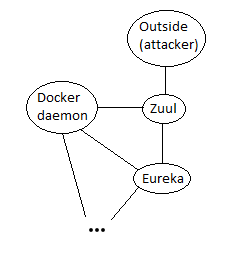
\includegraphics[width=.5\linewidth]{./images/Topology_graph}
		\caption{}
		\label{TopologyGraph}
	\end{subfigure}
	\hfill
	\begin{subfigure}[b]{\columnwidth}
		\centering
		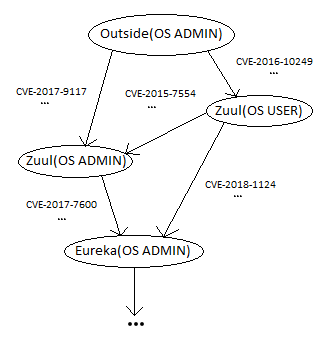
\includegraphics[width=.5\linewidth]{./images/Attack_graph}
		\caption{}
		\label{AttackGraph}
	\end{subfigure}
	
	\caption[Two numerical solutions]{Reduced Netflix OSS example (a) Example topology graph  (b) Example resulting attack graph}
\end{figure*}


In order to show how the attack graph generation works in practice, we present a small example. The example is taken from the Netflix OSS Github repository. Netflix OSS example is a Spring Cloud-based microservices architecture that enables Service Discovery (Eureka), Circuit Breaker (Hystrix), Intelligent Routing (Zuul) and Client Side Load Balancing (Ribbon) \cite{netflixoss, springcloudnetflix}. Displayed in Figure \ref{TopologyGraph} is a subset of the example topology where each node denotes a container and each edge denotes a connection between two containers. The topology consists of "Outside" node, "Docker daemon" node, Zuul, Eureka and other nodes. According to Netflix, Zuul is an edge service that provides dynamic routing, monitoring, resiliency, security, and more \cite{netflixzuul}, while Eureka is a REST (Representational State Transfer) based service that is primarily used in the AWS cloud for locating services for the purpose of load balancing and failover of middle-tier servers \cite{netflixeureka}. In Figure \ref{AttackGraph} we can see a part of the resulting attack graph, where a node corresponds to a pair of container plus its privilege, while an edge represents an atomic attack. Parts of both graphs have been intentionally omitted to reduce complexity. An example path that an attacker would take could be to first attack the Zuul container by exploiting the CVE-2016-10249 vulnerability by crafting an image file, which triggers a heap-based buffer overflow\footnote{\url{https://nvd.nist.gov/vuln/detail/CVE-2016-10249}} and gain USER privilege.  Then with this USER privilege, it can exploit the CVE-2015-7554 vulnerability on the same container via crafted field data in an extension tag in a TIFF image\footnote{\url{https://nvd.nist.gov/vuln/detail/CVE-2015-7554}} to gain ADMIN privilege. Once the ADMIN privilege has been obtained on Zuul, the attacker can attack the Eureka container by exploiting CVE-2017-7600 via another crafted image\footnote{\url{https://nvd.nist.gov/vuln/detail/CVE-2017-7600}} and gain ADMIN privilege. It is important to note that this is not the only path that the attacker can take in order to have ADMIN privileges on Eureka. Another path would be to exploit the CVE-2018-1124 vulnerability via creating entries in procfs by starting processes, which could result in crashes or arbitrary code execution\footnote{\url{https://nvd.nist.gov/vuln/detail/CVE-2018-1124}}. This vulnerability can be exploited by having only USER privilege on Zuul to gain directly ADMIN privileges of the Eureka container. Our attack graph generator shows both paths since it is of an interest to see every possible route in which a container can be compromised.



\subsection{Attack Graph Generation for Docker Networks}
\label{chap:technical}
 Figure \ref{AttackGraphSystem} gives an overview of the attack graph generator system. In the figure, the rectangles denote the main components of the system, while the arrows describe the flow of the system and the files are the intermediate products. Our attack graph generator is composed of three main components: Topology Parser, Vulnerability Parser and Attack Graph Parser. The Topology Parser reads the underlying topology of the system and converts it into to a format needed for our Attack Graph Parser, the Vulnerability Parser generates the vulnerabilities for each of the images and the Attack Graph Parser generates the attack graph from the topology and vulnerabilities files. 

In the following subsections, we first have a look into the system requirements, then describe each of the parsers in more detail and finally examine the characteristics of the Breath-first Search graph transversal algorithm.

\begin{figure}
	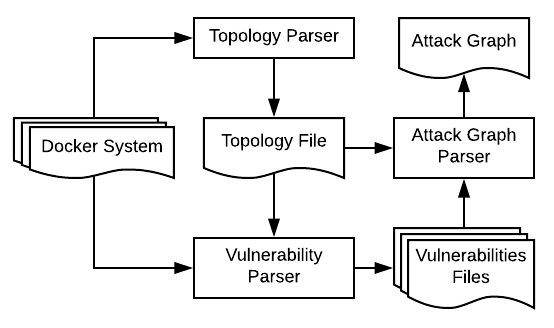
\includegraphics[scale=0.9]{./images/AttackGraphSystem}
	\caption{Overview of the Attack Graph Generator System}
	\label{AttackGraphSystem}
\end{figure}

Our system is developed for Docker 17.12.1-ce and Docker Compose 1.19.0 \cite{merkel2014docker}. Docker Compose is a tool for defining and running multi-container Docker applications \cite{dockercompose}. It provides a static configuration file that specifies the system containers, networks, ports etc. The code is written in Python 3.6, and we use Clair \cite{clair} and Clairctl \cite{clairctl} for vulnerabilities scanning.

We developed this system to be used with a specific version of Docker and Docker-Compose. This modular structure could, however, be easily extended to other versions of Docker-Compose, vulnerability scanners and microservice architectures by replacing the Vulnerability and Topology Parsers with custom ones and making sure that their outputs conform to the input of the Attack Graph Parser.

\subsubsection{Topology Parser}
\label{chap:topology_p}

In order to generate an attack graph of a given system, we require an arrangement of its components and connections described by a system topology. The topology of Docker containers can be described at either runtime or statically by using Docker Compose. In our case, since we are doing static attack graph analysis, we use Docker Compose as our main tool. Docker Compose provides a docker-compose.yml file which is used for extraction of the topology of the system. However different versions of docker-compose.yml, use different syntax. For example, older versions use the deprecated keyword "link", while newer ones use exclusively "networks", to denote a connection between two containers. In this work, we use the keyword "networks" as an indicator that a connection between two containers exists.

However, in the majority of cases, in order for an application to be useful, it has to communicate with the outside world. This is usually done by using publishing ports. This is the case in both computer networks, as well as in microservice architectures.

Another consideration that we take into account is the privileged access. Some containers require certain privileges over the docker daemon in order to function properly. For example, a user may want to run some hardware (web-cam \cite{webcam}) or some applications that demand higher privilege levels (Libvirt \cite{libvirt}) from Docker. In Docker, this is usually done either by mounting the Docker socket or specifying the keyword "privileged" in the docker-compose.yml file. An attacker with access to these containers has also access to the Docker daemon. Once the attacker has access to the Docker daemon, he has potential access to the whole microservice system, since every container is controlled and hosted by the daemon.

\begin{algorithm}
	\SetAlgoLined
	\KwData{topology, cont\_expl,
		priv\_acc}
	\KwResult{nodes, edges}
	nodes, edges, passed\_nodes = [], [], [] \\
	queue = Queue() \\
	queue.put("outside" + "ADMIN") \\
	
	\While{! queue.isEmpty()}{
		curr\_node = queue.get() \\
		curr\_cont = get\_cont(curr\_node) \\
		curr\_priv = get\_priv(curr\_node) \\
		neighbours = topology[curr\_cont] \\
		\For{neigh in neighbours}{
			\If{curr\_cont == docker\_host}
			{
				end = neigh + "ADMIN" \\
				create\_edge(curr\_node, end) \\
			}
			\If{neigh == docker\_host and priv\_acc[curr\_cont]}
			{     
				end = neigh + "ADMIN" \\
				create\_edge(curr\_node, end) \\
				queue.put(end) \\
				passed\_nodes.add(end)        
			}
			\If{neigh != outside and neigh != docker\_host}{
				precond = cont\_expl[neigh][precond] \\
				postcond = cont\_expl[neigh][postcond] \\
				\For{vul in vuls}{
					\If{$curr_priv > precond[vul]$}{    
						end = neigh + post\_cond[vul]\\
						create\_edge(curr\_node, end\_node)\\
						\If{end\_node not in passed\_nodes}{
							queue.put(end\_node)\\
							passed\_nodes.add(end\_node)
					}}
				}
			}
		}
		nodes = update\_nodes()\\
		edges = update\_edges() \\
	}
	
	\caption{BFS algorithm for attack graph generation}
	\label{BFSalgorithm}
\end{algorithm}



\subsubsection{Vulnerability Parser}
\label{chap:vulnerability_p}

In the preprocessing step, we use Clair to generate the vulnerabilities of a given container. Clair is a vulnerability scanner that inspects a Docker image and generates its vulnerabilities by providing CVE-ID, description and attack vector for each vulnerability \cite{clair}. An attack vector is an entity that describes which conditions and effects are connected to this vulnerability. The fields in the attack vector as described by the National Vulnerability Database(NVD) \cite{booth2013national} are: Access Vector (Local, Adjacent Network and Network), Access Complexity (Low, Medium, High), Authentication (None, Single, Multiple), Confidentiality Impact (None, Partial, Complete), Integrity Impact (None, Partial, Complete) and Availability Impact (None Partial, Complete). Unfortunately, Clair does not provide with a ready to use interface to analyze a docker image. As a result, we use Clairctl \cite{clairctl} in order to analyze a complete docker image.


\subsubsection{Attack Graph Generator}
\label{chap:attack_graph_p}

After the topology file is extracted and the vulnerabilities for each container are generated, we continue with the attack graph generation. Here, we first preprocess the vulnerabilities and convert them into sets of pre- and postconditions. In order to do this, we match the attack vectors acquired earlier from the vulnerability database and keywords of the descriptions of each vulnerability to generate attack rules. When a subset of attack vector fields and description keywords matches a given rule, we use the pre- or postcondition of that rule. If more than one rule matches, we take the one with the highest privilege level for the preconditions and the lowest privilege level for the postconditions. If no rule matches, we take None as a precondition and ADMIN(OS) as a postcondition. This results in a list of container vulnerabilities with their preconditions and postconditions.

\paragraph{Breadth-first Search}
\label{chap:bfs}

After the preprocessing step is done, the vulnerabilities are parsed and their pre- and postconditions are extracted. Together with the topology, they are feed into the Breadth-first Search algorithm (BFS).
Breadth-first Search is a popular search algorithm that traverses a graph by looking first at the neighbors of a given node, before diving deeper into the graph. Pseudocode of our modified Breadth-first Search is given in Algorithm \ref{BFSalgorithm}. The algorithm requires a topology and a dictionary of the exploitable vulnerabilities as an input and the output is made up of nodes and edges that make the attack graph. The algorithm first initializes the nodes, edges, queue and the passed nodes. Afterward, it generates the nodes which are a combination of the image name and the privilege level. Then into a while loop, it iterates through every node, checks its neighbors and adds the edges if the conditions are satisfied. If the neighbor was not passed, then it is added to the queue. The algorithm terminates when the queue is empty. Furthermore, BFS is characterized by the following properties:

\begin{table*}[t]
	\begin{center}
		\begin{tabular}{ p{20mm}p{35mm}p{35mm}p{10mm}cp{35mm} } 
			\hline
			Name & Description & Technology stack & No. Containers & No. vuln. & Github link \\\hline 
			
			Netflix OSS & Combination of containers provided from Netflix. & Spring Cloud, Netflix Ribbon, Spring Cloud Netflix, Netflix's Eureka & 10 & 4111 & \url{https://github.com/Oreste-Luci/netflix-oss-example} \\
			
			Atsea Sample Shop App & An example online store application. & Spring Boot, React, NGINX, PostgreSQL & 4 & 120 & \url{https://github.com/dockersamples/atsea-sample-shop-app} \\
			
			JavaEE demo & An application for browsing movies along with other related functions. & Java EE application, React, Tomcat EE & 2 & 149 & \url{https://github.com/dockersamples/javaee-demo} \\
			
			PHPMailer and Samba & An artificial example created from two separate containers. We use an augmented version for the scalability tests. & PHPMailer(email creation and transfer class for PHP), Samba(SMB/CIFS networking protocol) & 2 & 548 &  \url{https://github.com/opsxcq/exploit-CVE-2016-10033}
			\url{https://github.com/opsxcq/exploit-CVE-2017-7494} \\
			
			
			\hline
		\end{tabular}
	\end{center}
	
	\caption{Microservice architecture examples analyzed by the attack graph generator}
	\label{table_technologies}
	
\end{table*}

\begin{itemize}
	\item Completeness: Breadth-first Search is complete i.e. if there is a solution, Breadth-first search will find it regardless of the kind of graph.
	\item Termination: This follows from the monotonicity property. Monotonicity is ensured if it is assumed that an attacker will never need to relinquish a state \cite{ingols2006practical, ou2006scalable, ammann2002scalable}. In this implementation, each edge is traversed only once, making sure that monotonicity is preserved.
	\item Time Complexity: is $O(|N| + |E|)$ where $|N|$ is the number of nodes and $|E|$ is the number of edges in the attack graph.
\end{itemize}

\section{EVALUATION}
\label{chap:eval}

Real-world microservice systems comprise many containers that run different technologies with various degrees of connectivity among each other. This raises the need for a robust and scalable attack graph generator. We demonstrate use cases in Subsection \ref{chap:heterogenious_systems}. We then examine how others have evaluated their systems. In Subsection \ref{chap:scalability_eval}, we discuss experiments conducted to test the scalability of the proposed system with different numbers of containers and varying degrees of connectivity. Note that all experiments were performed on an Intel(R) Core(TM) i5-7200U CPU (2.50GHz) with 8 GB of RAM running Ubuntu 16.04.3 LTS.

\subsection{Use Cases}
\label{chap:heterogenious_systems}
\begin{table*}[!htb]
	\begin{center}
		\begin{tabular}{ p{20mm}p{35mm}p{35mm}p{10mm}cp{35mm} } 
			\hline
			Name & Description & Technology Stack & No. Containers & No. vuln. & GitHub link \\\hline 
			
			Netflix OSS & Combination of containers provided by Netflix. & Spring Cloud, Netflix Ribbon, Spring Cloud Netflix, Netflix's Eureka & 10 & 4111 & \url{https://github.com/Oreste-Luci/netflix-oss-example} \\
			
			Atsea Sample Shop App & An example online store application. & Spring Boot, React, NGINX, PostgreSQL & 4 & 120 & \url{https://github.com/dockersamples/atsea-sample-shop-app} \\
			
			JavaEE demo & An application for browsing movies along with other related functions. & Java EE application, React, Tomcat EE & 2 & 149 & \url{https://github.com/dockersamples/javaee-demo} \\
			
			PHPMailer and Samba & An artificial example created from two separate containers. We use an augmented version for the scalability tests. & PHPMailer(email creation and transfer class for PHP), Samba(SMB/CIFS networking protocol) & 2 & 548 &  \url{https://github.com/opsxcq/exploit-CVE-2016-10033}
			\url{https://github.com/opsxcq/exploit-CVE-2017-7494} \\
			
			
			\hline
		\end{tabular}
	\end{center}
	
	\caption{Microservice architecture examples analyzed by proposed attack graph generator}
	\label{table_technologies}
	
\end{table*}



Modern microservice architectures use many different technologies,  different numbers of containers, various degrees of connectivity, and have different numbers of vulnerabilities. Therefore, it is critically important to demonstrate that an attack graph generator works well in such heterogeneous scenarios. Here, we tested the proposed system on real and slightly modified GitHub examples (Table \ref{table_technologies}). We employed test examples that are publicly available to facilitate potential future comparison characterized by different system properties (e.g., topologies, technologies and vulnerabilities) and different usage domains. We also had to consider the fact that an overwhelming majority of publicly-available examples are small, i.e., only one or a few containers, which made finding appropriate test examples challenging. The resulting examples are as follows:

\begin{itemize}
	\item NetflixOSS is a microservice system provided by Netflix comprising 10 containers and uses many tools, e.g., Spring Cloud, Netflix Ribbon, and Netflix Eureka.
	\item The Atsea Sample Shop App is an e-commerce sample web application comprising four containers and uses Spring Boot, React, NGINX, and PostgreSQL.
	\item The JavaEE demo is a sample application for browsing movies comprising only two containers and uses JavaEE, React, and Tomcat EE.
\end{itemize}

   We ran the attack graph generator and manually verified the resulting attack graphs for the small examples based on domain knowledge under the assumption that the output from Clair, the NVD attack vectors \cite{booth2013national}, and the preconditions and postconditions from Aksu et al. \cite{aksu2018automated} are \textit{correct}. After running the proposed attack graph generator, the attack graphs for the Atsea Sample Shop App and JavaEE demo were small as expected, containing only a few nodes and edges. The structure of the NetflixOSS attack graph demonstrated a nearly linear structure in which each node was connected to a small number of other nodes to form a chain of attacks. This linearity is due to the fact that each container is connected to only a few other containers to reduce unnecessary communication and increase encapsulation. Therefore, based on this degree of connectivity, an attacker needs to perform multiple intermediate steps to reach the target container. Note that all examples terminated, there were no directed edges from containers with higher privileges to lower privileges, no duplication of nodes, and no reflexive edges were observed, which is in line with the monotonicity property. In addition, the run time of the proposed system with each example was short, however, additional scalability tests were required. Therefore, the Phpmailer and Samba system was extended and employed as an artificial example to perform scalability tests. This is discussed in the following subsection.



\subsection{Scalability evaluation}
\label{chap:scalability_eval}


\begin{table*}
	\begin{center}
		\begin{tabular}{ cccccc } 
			\hline
			Statistics & example\_20 & example\_50 & example\_100 & example\_500 & example\_1000 \\ \hline
			
			No. of Phpmailer containers & 1 & 1 & 1 & 1 & 1 \\ 
			
			No. of Samba containers & 20 & 50 & 100 & 500 & 1000 \\ 
			
			No. of nodes in topology & 23 & 53 & 103 & 503 & 1003\\ 
			
			No. of edges in topology & 253 & 1378 & 5253 & 126253 & 502503 \\ 
			
			No. nodes in attack graph & 43 & 103 & 203 & 1003 & 2003 \\ 
			
			No. edges in attack graph & 863 & 5153 & 20303 & 501503 & 2003003 \\ 
			
			Topology parsing time & 0.02879 & 0.0563 & 0.1241 & 0.7184 & 2.3664 \\ 
			
			Vulnerability preprocessing time & 0.5377 & 0.9128 & 1.6648 & 6.9961 & 15.0639 \\ 
			
			BFS time & 0.2763 & 1.6524 & 6.5527 & 165.3634 & 767.5539 \\ 
			
			Total time & 0.8429 & 2.6216 & 8.3417 & 173.0781 & 784.9843 \\ 
			\hline
		\end{tabular}
	\end{center}
	
	\caption{Scalability results with graph characteristics and execution times (s)}
	
	\label{table_scalability}
\end{table*}
Extensive study of the scalability of attack graph generators is rare in the current literature, and many parameters contribute to the complexity of comprehensive analyses. Parameters that typically vary in this sort of evaluation include the number of nodes, their connectivity and the number of vulnerabilities per container, all of which contribute to the execution time of a given algorithm. Even though the definitions of an attack graph differ, we hope to achieve a comprehensive comparison with current methods. Here, we compared the proposed system to existing work in computer networks by treating each container as a host machine and any physical connection between two machines as a connection between two containers. In the following, we first examine three methods and their scalability evaluation results. We then present the scalability results of the proposed system.

Sheyner et al. \cite{sheyner2002automated} tested their system (NuSMV) using both small and extended examples. The attack graph in the larger example has 5948 nodes and 68364 edges. The time required for NuSMV to execute this configuration was two hours; however, the model checking component took four minutes. The authors claim that the performance bottleneck resides in the graph generation procedure. Ingols et al. \cite{ingols2006practical} tested their system on a network of 250 hosts. They continued the study on a simulated network with 50000 hosts in under four minutes. Although their method yields better performance than NuSMV, their evaluation was based on a MP graph, which differs from our target graph. Ou et al. \cite{ou2006scalable} provided a more extensive study, wherein they tested their system (MulVAL) using more examples. They state that the asymptotic CPU time was between $O(n^2)$ and $O(n^3)$, where n is the number of nodes (hosts). With 1000 fully-connected nodes, their system required more than 1000 seconds to execute. % The authors also provide an evaluation where he MulVAL clearly outperforms the Sheyner's system.

We used Samba \cite{samba} and Phpmailer \cite{phpmailer} containers in our scalability experiments. We extended this example and artificially created fully-connected topologies of \textit{20, 50, 100, 500, and 1000} Samba containers to test the scalability of the proposed system. As reported by Clair, the Phpmailer container has \textit{181} vulnerabilities and the Samba container has \textit{367} vulnerabilities. In our tests, we measured the total execution time and partial times, i.e., topology parsing time, vulnerability preprocessing time, and BFS time. The total time contains topology parsing, attack graph generation, and other utility processes. Here, the topology parsing time is the time required to generate the graph topology, the vulnerability preprocessing time is the time required to convert vulnerabilities into sets of preconditions and postconditions, and the BFS time is the time required for the BFS algorithm to traverse the topology and generate the attack graph after the previous steps are complete. All components were executed five times for each example and their final time was averaged. Note that the measured times are given in seconds.  However, the total time does not include the Clair vulnerability analysis, because this evaluation is beyond the scope of this analysis.

Table \ref{table_scalability} shows the experimental results. In each experiment, the number of Phpmailer containers was constant. In contrast, the number of Samba containers increased in a fully-connected manner, where a node of each container was connected to all other containers. In addition, there were also two additional artificial containers, i.e., "outside," which represents the environment from where the attacker can attack, and the "docker host," i.e., the Docker daemon where containers are hosted. Thus, the total number of nodes in the topology graph is the sum of "outside," "docker host," the number of Phpmailer containers, and the number of Samba containers. The number of edges in the topology graph is a combination of one edge ("outside"-"Phpmailer"), n edges ("docker host" to all containers) and n*(n+1)/2 edges between the Phpmailer and Samba containers. For example\_20, the number of containers is 23 (one Phpmailer container, one "outside" container, one "docker host" container, and 20 Samba containers). Thus, the number of edges in this topology graph is 253, i.e., one outside edge, 21 Docker host edges (one toward Phpmailer and 20 toward the Samba containers), and 231 between-container edges (i.e., 21*22/2=231).

Throughout the experiments, the greatest time bottleneck was the preprocessing step for the smaller configurations. However, this time increased linearly because the container files are analyzed only once by Clair. Note that the attack graph generation time for the smaller examples was considerably less than the preprocessing time. For example\_500, we note a sharp increase in execution time (165 seconds) compared to the previous example (i.e., example\_100), where the attack graph was generated in 6.5 seconds.

The total time of the attack graph generation procedure for 1000 fully-connected hosts (784 seconds) was better than the results of Ou et al. \cite{ou2006scalable}, i.e., 1000 seconds. In Sheyners's extended example (four hosts, eight atomic attacks and multiple vulnerabilities), the attack graph took two hours to create. In contrast, even for a greater number of hosts (1000), the proposed attack graph procedure demonstrates faster attack graph generation time. However, the proposed system performs worse than the generator proposed by Ingols et al., but that is attributed to the usage of the MP attack graph, which differs from our target graph. 

In summary, we found that the proposed algorithm generates attack graphs efficiently, i.e., it handles a system with 1000 containers in 13 minutes. Considering the strongly-connected system employed in the experiment and the high number of vulnerabilities in this system, we consider that the results demonstrate that the proposed system is a practical solution that can be used as part of the continuous delivery processes of real-world systems. 
\section{RELATED WORK}
\label{chap:related_work}

Previous work has dealt with attack graph generation, mainly in computer networks \cite{ingols2006practical, sheyner2002automated, ritchey2000using, ou2006scalable}, where multiple machines are connected to each other and the Internet. %In these networks, an attacker performs multiple steps to achieve his goal, i.e., gaining privileges of a specific host. Attack graphs help in analyzing this behavior. Although attack graphs are useful, constructing them manually can be a cumbersome and time-consuming process. Tools that generate vulnerabilities of a specific host are available \cite{clair, artz2002netspa, farmer1990cops}. However previous works state that these tools alone are not enough to analyze the vulnerability of an entire network and that these tools in addition to network topology could solve this issue. This outcome is because different hosts are connected together and influence the outcome of an attack. Therefore, some teams have been working on developing systems that generate attack graphs automatically by using different approaches.
One of the earlier works in attack graph generation was done by Sheyner et al. by using model checkers with goal property \cite{sheyner2002automated}. Model checkers use computational logic to check if a model is correct, and otherwise, they provide a counterexample. A collection of these counterexamples form an attack graph. They state that model checkers satisfy a monotonicity property  to ensure termination. However, model checkers have a computational disadvantage. %In the example provided, NuSMV takes 2 hours to construct the attack graph with 5948 nodes and 68364 edges . As a result of this, more scalable approach was needed.
 Amman et al. extend this work with some simplifications and more efficient storage \cite{ritchey2000using}. Ou et al. use a logical attack graph \cite{ou2006scalable} and Ingols \cite{ingols2006practical} et al. use a Breadth-first search algorithm in order to tackle the scalability issue. Ingols et al. discuss the redundancy Full and Predictive graphs and model an attack graph as an MP graph with content-less edges and 3 types of nodes. They use Breath-first search technique to generate the attack graph. This approach provides faster results in comparison to using model checkers. An MP graph of 8901 nodes and 23315 edges is constructed in 0.5 seconds. Aksu et al. build on top of Ingols's system and evaluate a set of rule pre- and postconditions in generating attacks. They define a specific test of pre- and postcondition rules and test their correctness. In their evaluation, they use a machine learning approach \cite{aksu2018automated}.

Containers and microservice architectures, despite their ever-growing popularity, have shown somewhat bigger security risks, mostly because of their  need of connectivity and a lesser degree of encapsulation \cite{combe2016docker, dragoni2017microservices}. To the best of our knowledge, no previous work that has been done  in the area of attack graph generation for Docker containers. Similar to computer networks, microservice architectures have a container topology and tools for analysis of containers. Containers in our model correspond to hosts, and a connection between hosts translates to communication between containers. 

In summary, our contribution is proposing attack graph generation as part of the DevOps practices, and providing a tool-support for this idea. To that end, we extended the work from Ingols \cite{ingols2006practical} and Aksu \cite{aksu2018automated} in conjunction with Clair OS to generate attack graphs for microservice architectures. 


\section{CONCLUSIONS AND FUTURE WORK}
\label{chap:conclusion}

Microservices are a promising architectural style that advocate practitioners to build systems as a group of small connected  services. Although this style enables better scalability and faster deployment, the full container-based automation within this style raises many security concerns. In this paper, we proposed to use automated attack graph generation as part of the practices of developing microservice-based architectures. Attack graphs aid the developers in identifying attack paths that consist of multiple vulnerability exploitation in the deployed services. The manual construction of attack graphs is an error-prone, resource consuming activity. Hence, automating this process does not only guarantee efficient construction but also complies with the spirit of DevOps practices. We have shown that such automation, extending previous works in computer networks field, is efficient and scales to complex and big microservice-based systems. 

As a future work, we plan to extend this work to support more frameworks that are used in microservices systems. We also plan to study the possible analysis of the resulting attack graphs for purposes of attack detection, and post-postmortem forensics investigations. 
\bibliographystyle{ACM-Reference-Format}
\bibliography{sample-bibliography} 

\end{document}
